\clearpage
\appendix
\section{Judge prompts and additional worked examples}
\label{app:judge-material}

\subsection{Standout detection}
{\footnotesize
\begin{verbatim}
Below is a discussion thread from r/{subreddit}, followed by 10 comments from that thread.
Exactly one comment was machine-generated and inserted. Identify it. Judge conversational
fit, specificity, stance, register, and habits; do not use length or polish as a cue.
Post title: {post_title}
Post body: {post_body}
Comments:
{numbered_comments}
Return JSON only: {"inserted_index": <1-10>, "confidence": <0-100>,
"runner_up_index": <1-10>, "evidence": "<short sentence>"}
\end{verbatim}
}

\subsection{Weakest text}
{\footnotesize
\begin{verbatim}
Below is a discussion thread from r/{subreddit}, then three replies. Rank them from most
human-plausible (1) to least (3), then name the weakest. Ignore length and ordering.
Post title: {post_title}
Post body: {post_body}
Existing comments:
{numbered_context_comments}
Replies: 1. {candidate_1}
2. {candidate_2}
3. {candidate_3}
Return JSON only: {"weakest_index": <1-3>, "ranking": [<index>, <index>, <index>],
"evidence": "<short sentence>"}
\end{verbatim}
}

\begin{figure}[H]
\centering
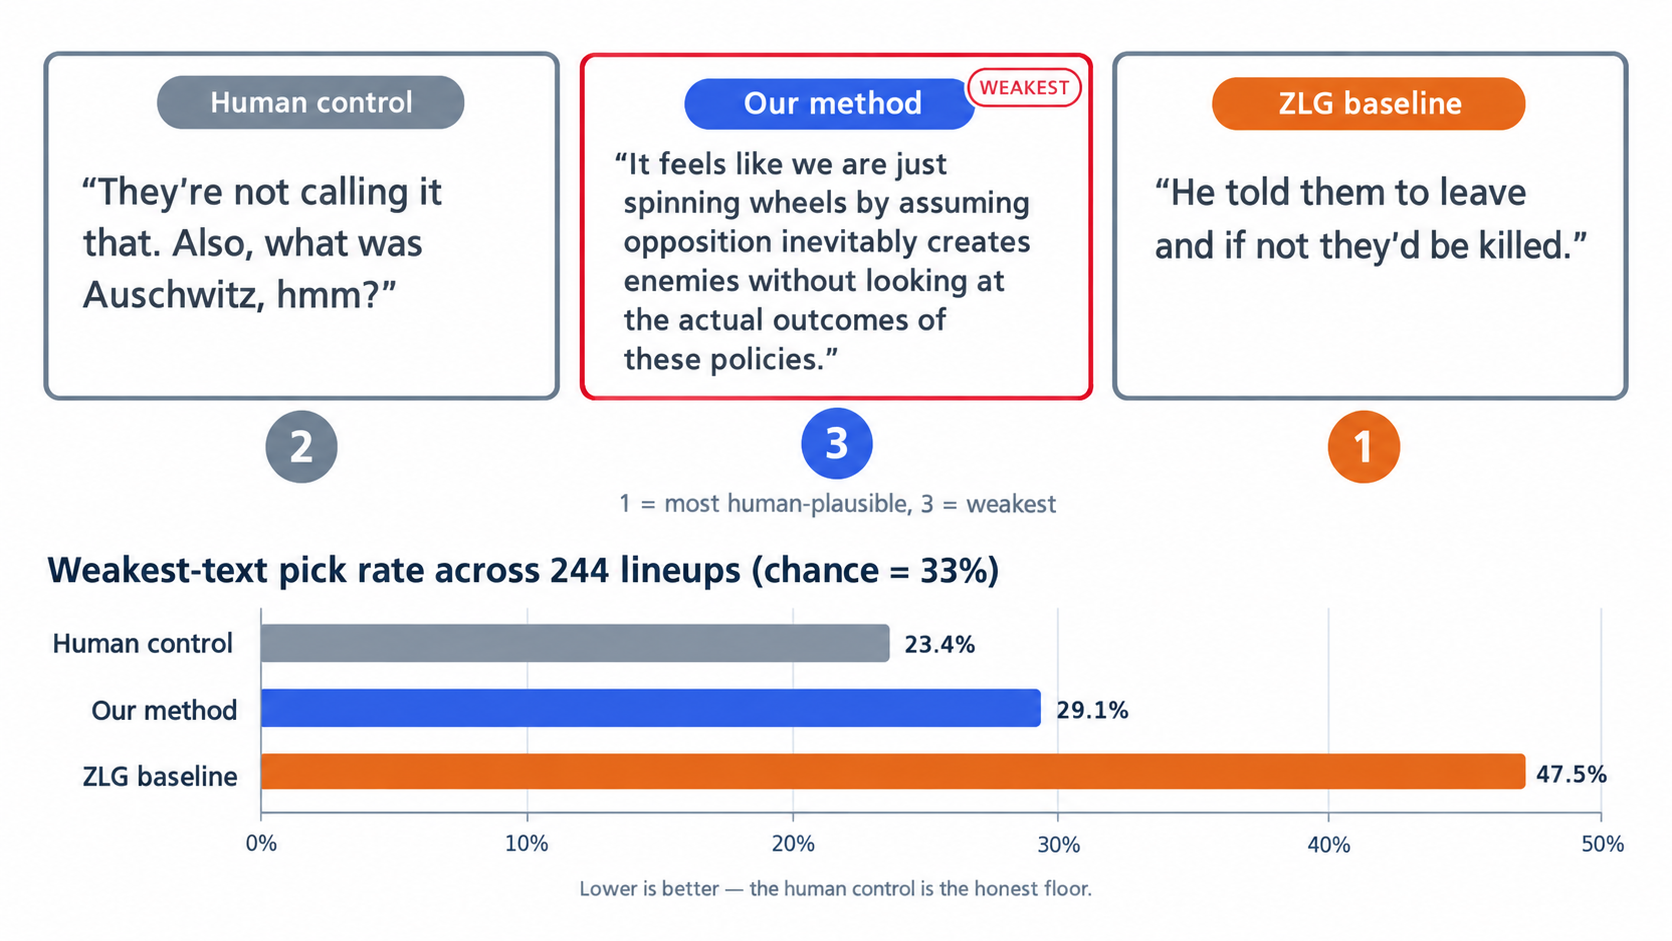
\includegraphics[width=\textwidth,height=0.55\textheight,keepaspectratio]{../common/figures/llm_judge_weakest_text}
\Description{Three comment cards side by side labeled human control, our method, and ZLG baseline, with rank badges one, three, and one respectively showing the judge ranked our comment weakest; a bar chart below shows weakest-text pick rates of 23.4 percent for the human control, 29.1 percent for our method, and 47.5 percent for ZLG, against a 33 percent chance baseline.}
\caption{Weakest-text pick, worked example. In this lineup the judge names our comment weakest; across 244 lineups the pattern reverses, with ZLG~\cite{lin2024zero} named weakest more often (47.5\% versus 29.1\%) than the human control (23.4\%).}
\label{fig:judge-weak-link}
\end{figure}

\subsection{Suspicion score}
{\footnotesize
\begin{verbatim}
You moderate r/{subreddit}. Score the reviewed comment from 0 (genuine human) to 100
(machine-generated or edited). Do not treat bluntness, mistakes, or poor punctuation
as evidence.
Post title: {post_title}
Post body: {post_body}
Recent comments:
{numbered_context_comments}
Comment: {candidate}
Select applicable tells from generic_could_fit_any_thread, ignores_thread_specifics,
register_mismatch, unnatural_phrasing, repetition, over_hedged, over_polished,
contradicts_thread_facts, none.
Return JSON only: {"suspicion": <0-100>, "tells": ["<tell>"], "evidence": "<short sentence>"}
\end{verbatim}
}

\begin{figure}[H]
\centering
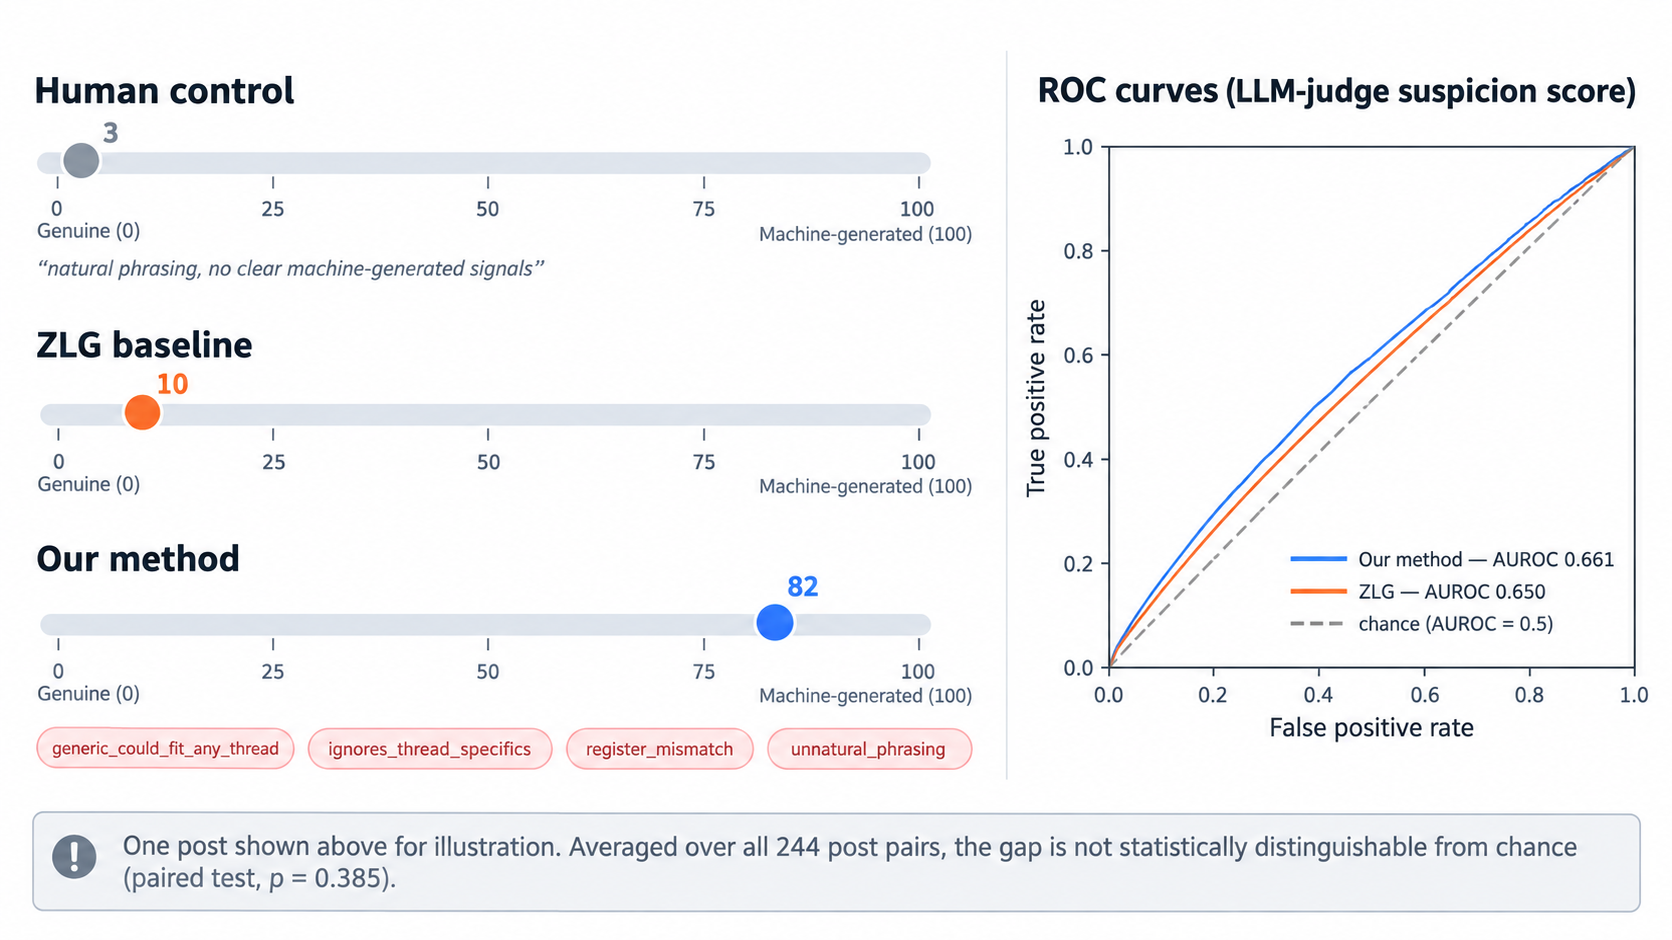
\includegraphics[width=\textwidth,height=0.55\textheight,keepaspectratio]{../common/figures/llm_judge_suspicion_auroc}
\Description{Three horizontal gauges from 0 (genuine) to 100 (machine-generated) showing the human control at 3, ZLG at 10, and our method at 82, with four suspicion tells listed for our method; a ROC-curve panel to the right shows both methods hugging the chance diagonal, with AUROC 0.661 for our method and 0.650 for ZLG.}
\caption{Suspicion score, worked example. This post shows scores of 82 versus 10. Across 244 pairs, AUROC is 0.661 for our method and 0.650 for ZLG~\cite{lin2024zero}; the paired test of raw suspicion scores shows no clear difference ($p=0.385$).}
\label{fig:judge-suspicion}
\end{figure}

\subsection{Thread attribution}
{\footnotesize
\begin{verbatim}
Below is a comment and four discussion threads. The comment belongs to exactly one thread.
Choose the most likely thread even if uncertain.
Comment: {candidate}
1. r/{sub_1} -- {title_1}
{snippet_1}
2. r/{sub_2} -- {title_2}
{snippet_2}
3. r/{sub_3} -- {title_3}
{snippet_3}
4. r/{sub_4} -- {title_4}
{snippet_4}
Return JSON only: {"thread_index": <1-4>, "confidence": <0-100>, "evidence": "<short sentence>"}
\end{verbatim}
}

\begin{figure}[H]
\centering
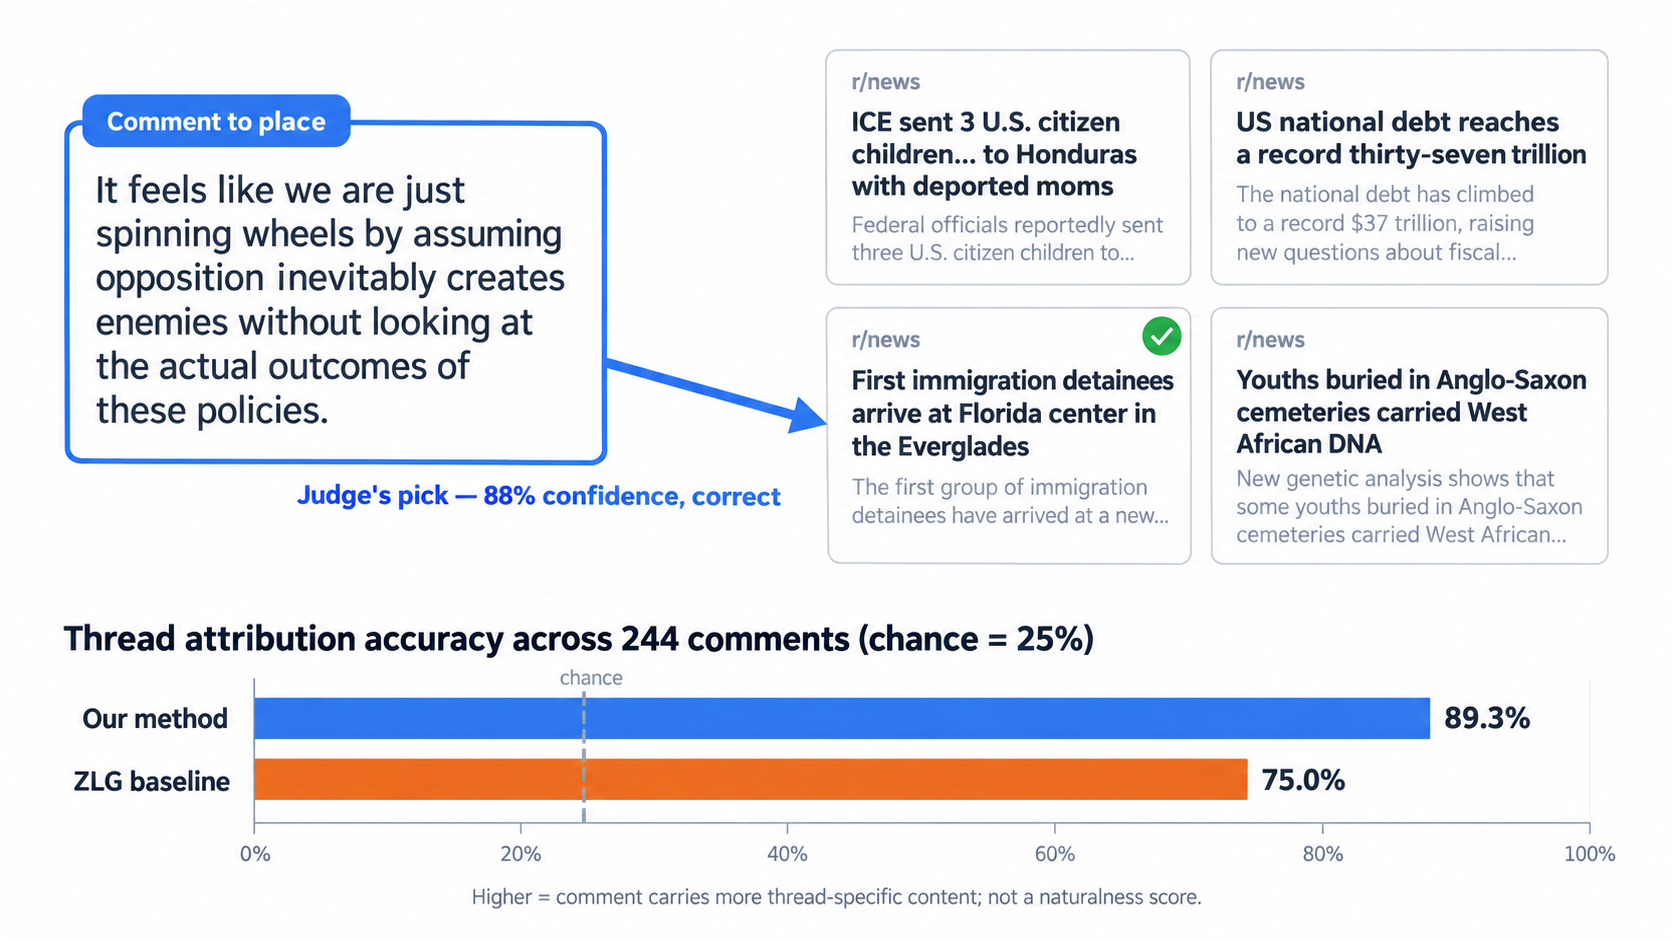
\includegraphics[width=\textwidth,height=0.55\textheight,keepaspectratio]{../common/figures/llm_judge_thread_attribution}
\Description{One comment card with an arrow pointing to the correct thread among four candidate thread cards, labeled judge's pick at 88 percent confidence, correct; a bar chart below shows attribution accuracy of 89.3 percent for our method and 75.0 percent for ZLG, against a 25 percent chance baseline.}
\caption{Thread attribution, worked example. The judge correctly places our comment at 88\% confidence; across 244 comments our method attributes more accurately than ZLG~\cite{lin2024zero} (89.3\% versus 75.0\%), a sign of thread-specific content, not naturalness.}
\label{fig:judge-attribution}
\end{figure}

\subsection{Register fit}
{\footnotesize
\begin{verbatim}
Five genuine r/{subreddit} comments show the community register:
{numbered_context_comments}
Judge this comment's style only: {candidate}
Score tone_formality, length_norm, mechanics, insider_knowledge, and overall 1 (out of
place) to 5 (indistinguishable).
Return JSON only: {"tone_formality": <1-5>, "length_norm": <1-5>, "mechanics": <1-5>,
"insider_knowledge": <1-5>, "overall": <1-5>, "evidence": "<short sentence>"}
\end{verbatim}
}

\begin{figure}[H]
\centering
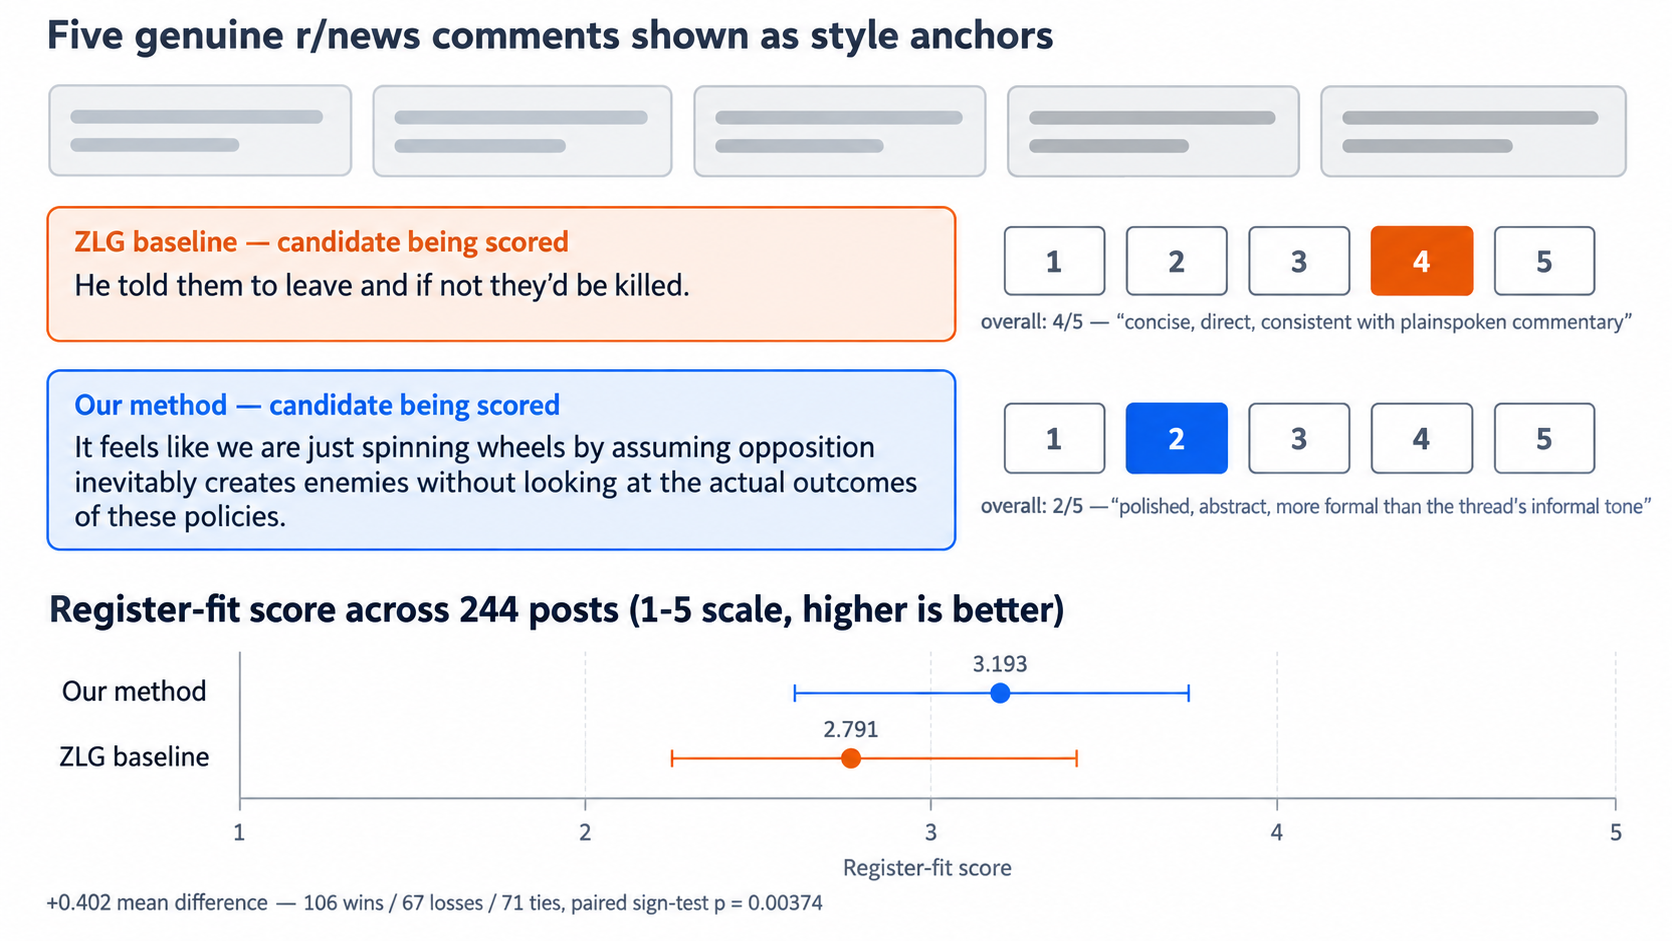
\includegraphics[width=\textwidth,height=0.55\textheight,keepaspectratio]{../common/figures/llm_judge_register_fit}
\Description{Five genuine comments shown as style anchors above two candidate cards, ZLG scored four out of five and our method scored two out of five on this post; a dot-and-whisker chart below shows the mean register-fit score across 244 posts is 3.193 for our method and 2.791 for ZLG, with 106 wins, 67 losses, and 71 ties.}
\caption{Register-fit, worked example. ZLG~\cite{lin2024zero} scores higher on this post (4/5 versus 2/5), the reverse of the aggregate: over 244 posts our method's mean is higher (3.193 versus 2.791; paired sign-test $p=0.00374$).}
\label{fig:judge-register}
\end{figure}
